%\newsection{Kapitel1}

%Hier den Inhalt mit \input einfügen und die folgenden Zeilen entfernen


%%%%%%%%%%%%%%%%%%%%%%%%%%%%%%%%%%%%%%%%%%%%%%%%% Anfang - Kapazität	 %%%%%%%%%%%%%%%%%%%%%%%%%%%%%%%%%%%%%%%%%%%%%%

	\section{Kapazität und Kondensator}
\s{
In der Elektrotechnik gibt es drei grundlegende Komponenten, mit denen das elektrische Verhalten von Bauteilen beschrieben werden kann.
Neben dem zuvor behandelten ohmschen Widerstand, gibt es noch die Kapazität und die Induktivität.
In diesem Abschnitt geht es um die Eigenschaft der Kapazität, sowie dem dazugehörigen Bauteil, dem Kondensator.
Der darauffolgende Abschnitt behandelt die Induktivität sowie das zugehörige Bauteil, die Spule.
}
%%%%%%%%%%%%%%%%%%%%%%%%%%%%%%%%%%%%%%%%%%%%%%%%% Anfang - Lernziele Kapazität	 %%%%%%%%%%%%%%%%%%%%%%%%%%%%%%%%%%%%%%%%%%%%%%
\begin{frame}
	\ftx{Lernziele: Kapazität und Kondensator}
\begin{Lernziele}{Kapazität und Kondensator}
	Die Studierenden
	\begin{itemize}
	\item können zwischen Kapazität und Kondensator differenzieren.
	\item kennen die wichtigsten Parameter rund um den Kondensator und die Kapazität.
	\item können die Kapazität eines Kondensators berechnen.
\end{itemize}
\end{Lernziele}
\end{frame}

%%%%%%%%%%%%%%%%%%%%%%%%%%%%%%%%%%%%%%%%%%%%%%%%% Ende - Lernziele Kapazität	 %%%%%%%%%%%%%%%%%%%%%%%%%%%%%%%%%%%%%%%%%%%%%%

	\subsection{Die elektrische Kapazität $C$}
\s{
	Die elektrische Kapazität ist die Fähigkeit eines Objektes, elektrische Energie in Form eines elektrischen Feldes, zu speichern.
	Diese Eigenschaft kommt zustande, sobald elektrische Ladungsträger ungleich verteilt sind und sich zwischen den Bereichen
	ein elektrisches Feld ausbildet. Das Formelzeichen der Kapazität ist $C$ (capacity) während die Einheit in Farad ($F$) angegeben wird.

}% nur im Skript

\s{
Das einfachste und geläufigste Beispiel, an dem die Kapazität erklärt werden kann, ist der Plattenkondensator.
Bei dieser Art des Kondensators liegen sich zwei leitfähige Platten gegenüber, welche jeweils mit einem anderen Potential beaufschlagt werden.
In Abbildung \ref{fig:idealer Kondensator} ist ein Kondensator mit idealisiertem Feldverlauf dargestellt.
}
%%%%%%%%%%%%%%%%%%%%%%%%%%%%%%%%%%%%%%%%%%%%%%%%% Anfang - Grafik idealer Kondensator	 %%%%%%%%%%%%%%%%%%%%%%%%%%%%%%%%%%%%%%%%%%%%%%
\begin{frame}
	\ftx{Die elektrische Kapazität}
	\b{
		\begin{itemize}
			\item Der ideale Plattenkondensator
			\end{itemize}
	}
	\begin{figure}[H]
		\centering
			\includesvg[width=0.6\textwidth]{Idealer_Plattenkondensator.svg}
			\s{\caption{\textbf{Idealer Plattenkondensator mit idealisierten Feldverlauf.} Der Kondensator
			speichert elektrische Energie in einem elektrischen Feld was idealisiert zwischen den Platten dargestellt ist und hat eine konstante Kapazität \( C \), die nur von der Fläche der Platten und dem Abstand zwischen ihnen abhängt.}}
			\label{fig:idealer Kondensator}
		\end{figure}
%%%%%%%%%%%%%%%%%%%%%%%%%%%%%%%%%%%%%%%%%%%%%%%%% Ende - Grafik idealer Kondensator	 %%%%%%%%%%%%%%%%%%%%%%%%%%%%%%%%%%%%%%%%%%%%%%
\s{
Aufgrund der unterschiedlichen Potentiale auf den Platten, bildet sich von der höheren zur geringer geladenen Platte ein elektrisches Feld aus.
Im idealen Fall wird angenommen, dass sich außerhalb der Kondensatorplatten kein Feld ausbildet.
In der Realität sammeln sich an den seitlichen Rändern der Platten ebenfalls Ladungsträger, welche zu komplizierteren Feldverteilungen führen.
In Abbildung \ref{fig:realer Kondensator} ist die Grafik eines solchen realen Plattenkondensators dargestellt.
}% nur im Skript
\end{frame}
%%%%%%%%%%%%%%%%%%%%%%%%%%%%%%%%%%%%%%%%%%%%%%%%% Anfang - Grafik realer Kondensator	 %%%%%%%%%%%%%%%%%%%%%%%%%%%%%%%%%%%%%%%%%%%%%%
\begin{frame}
	\ftx{Die elektrische Kapazität}
	\b{
		\begin{itemize}
			\item Der reale Plattenkondensator
			\end{itemize}
	}
	\begin{figure}[H]
		\centering
			\includesvg[width=0.6\textwidth]{Realer_Plattenkondensator.svg}
			\s{\caption{\textbf{Realer Kondensator mit realem Feldverlauf.} Im Gegensatz zum idealen Kondensator treten
			  Randfelder und Verluste auf, die die tatsächliche Kapazität und das elektrische Verhalten beeinflussen.}}

			\label{fig:realer Kondensator}
		\end{figure}
\end{frame}
%%%%%%%%%%%%%%%%%%%%%%%%%%%%%%%%%%%%%%%%%%%%%%%%% Ende - Grafik realer Kondensator	 %%%%%%%%%%%%%%%%%%%%%%%%%%%%%%%%%%%%%%%%%%%%%%
\begin{frame}[t]
	\ftx{Die elektrische Kapazität}
\b{
	\begin{minipage}[t]{1\textwidth}
	\begin{equation*}
		[C] =  1\, \text{Farad} = 1\, \text{F} =  1\,\, \frac{\text{C}}{\text{V}} = 1\, \frac{\text{A} \text{s}}{\text{V}} \label{eq:cqu}
	\end{equation*}
	\vspace{0.1cm}
	\begin{equation*}
		C = \frac{Q}{U}
	\end{equation*}
	\end{minipage}
%%% aus Einführung in zeitabhängige Vorgänge (MH)
	\vspace{2cm}
	\only<2->{\begin{equation*}
		Q = C \cdot U \quad \Rightarrow \quad C = \frac{Q}{U} = \frac{\varepsilon \cdot \iint \vec{E} \cdot \mathrm{d}\vec{A}}{\int \vec{E}\mathrm{d}\vec{s}}
	\end{equation*}}
}
\end{frame}
\s{
	In vielen Fällen kann das reale Verhalten jedoch vernachlässigt werden, was die Berechnungen deutlich vereinfacht.
	Aus dem Grund wird im Folgenden nurnoch von idealisierten Kondensatoren ausgegangen.


	Die Kapazität ist definiert als das Verhältnis der gespeicherten elektrischen Ladung $Q$ zur angelegten Spannung $U$.
	Je höher die Kapazität eines Kondensators ist, desto mehr Ladung kann er bei einer gegebenen Spannung speichern.

%%%%%%%%%%%%%%%%%%%%%%%%%%%%%%%%%%%%%%%%%%%%%%%%% Anfang - Formeln Kapazität	 %%%%%%%%%%%%%%%%%%%%%%%%%%%%%%%%%%%%%%%%%%%%%%
	\begin{equation*}
		[C] =  1\, \text{Farad} = 1\, \text{F} =  1\,\, \frac{\text{C}}{\text{V}} = 1\, \frac{\text{A} \text{s}}{\text{V}} \label{eq:cqu}
	\end{equation*}
	\vspace{0.1cm}
	\begin{equation}
		C = \frac{Q}{U}
	\end{equation}
%%% aus Einführung in zeitabhängige Vorgänge (MH)
	\begin{equation}
		Q = C \cdot U \quad \Rightarrow \quad C = \frac{Q}{U} = \frac{\varepsilon \cdot \iint \vec{E} \cdot \mathrm{d}\vec{A}}{\int \vec{E}\mathrm{d}\vec{s}} \label{eq:qcu2}
	\end{equation}
}

%%%%%%%%%%%%%%%%%%%%%%%%%%%%%%%%%%%%%%%%%%%%%%%%% Ende - Formeln Kapazität	 %%%%%%%%%%%%%%%%%%%%%%%%%%%%%%%%%%%%%%%%%%%%%%
	\subsection{Der Kondensator als Bauelement}

\s{
	Die Eigenschaften der Kapazität werden in verschiedenen Bereichen der Elektrotechnik bewusst genutzt.
	Die Nutzbarmachung dieser Eigenschaften erfolgt mit Hilfe von Kondensatoren. Es gibt sie in verschiedenen Ausführungen.
	Abbildung \ref{fig:Verschiedene Kondensatoren} zeigt einige Beispiele von THT- bis hin zu SMD-Bauteilen.
}

%%%%%%%%%%%%%%%%%%%%%%%%%%%%%%%%%%%%%%%%%%%%%%%%% Anfang - Bild versch. Kondensatoren	%%%%%%%%%%%%%%%%%%%%%%%%%%%%%%%%%%%%%%%%%%%%%%

%%% Quelle einfügen!

\begin{frame}
	\ftx{Der Kondensator als Bauelement}
	\b{
		\begin{itemize}
			\item Verschiedene Arten und Bauformen von Kondensatoren
		\end{itemize}
	}
	\begin{figure}[H]
		\centering
		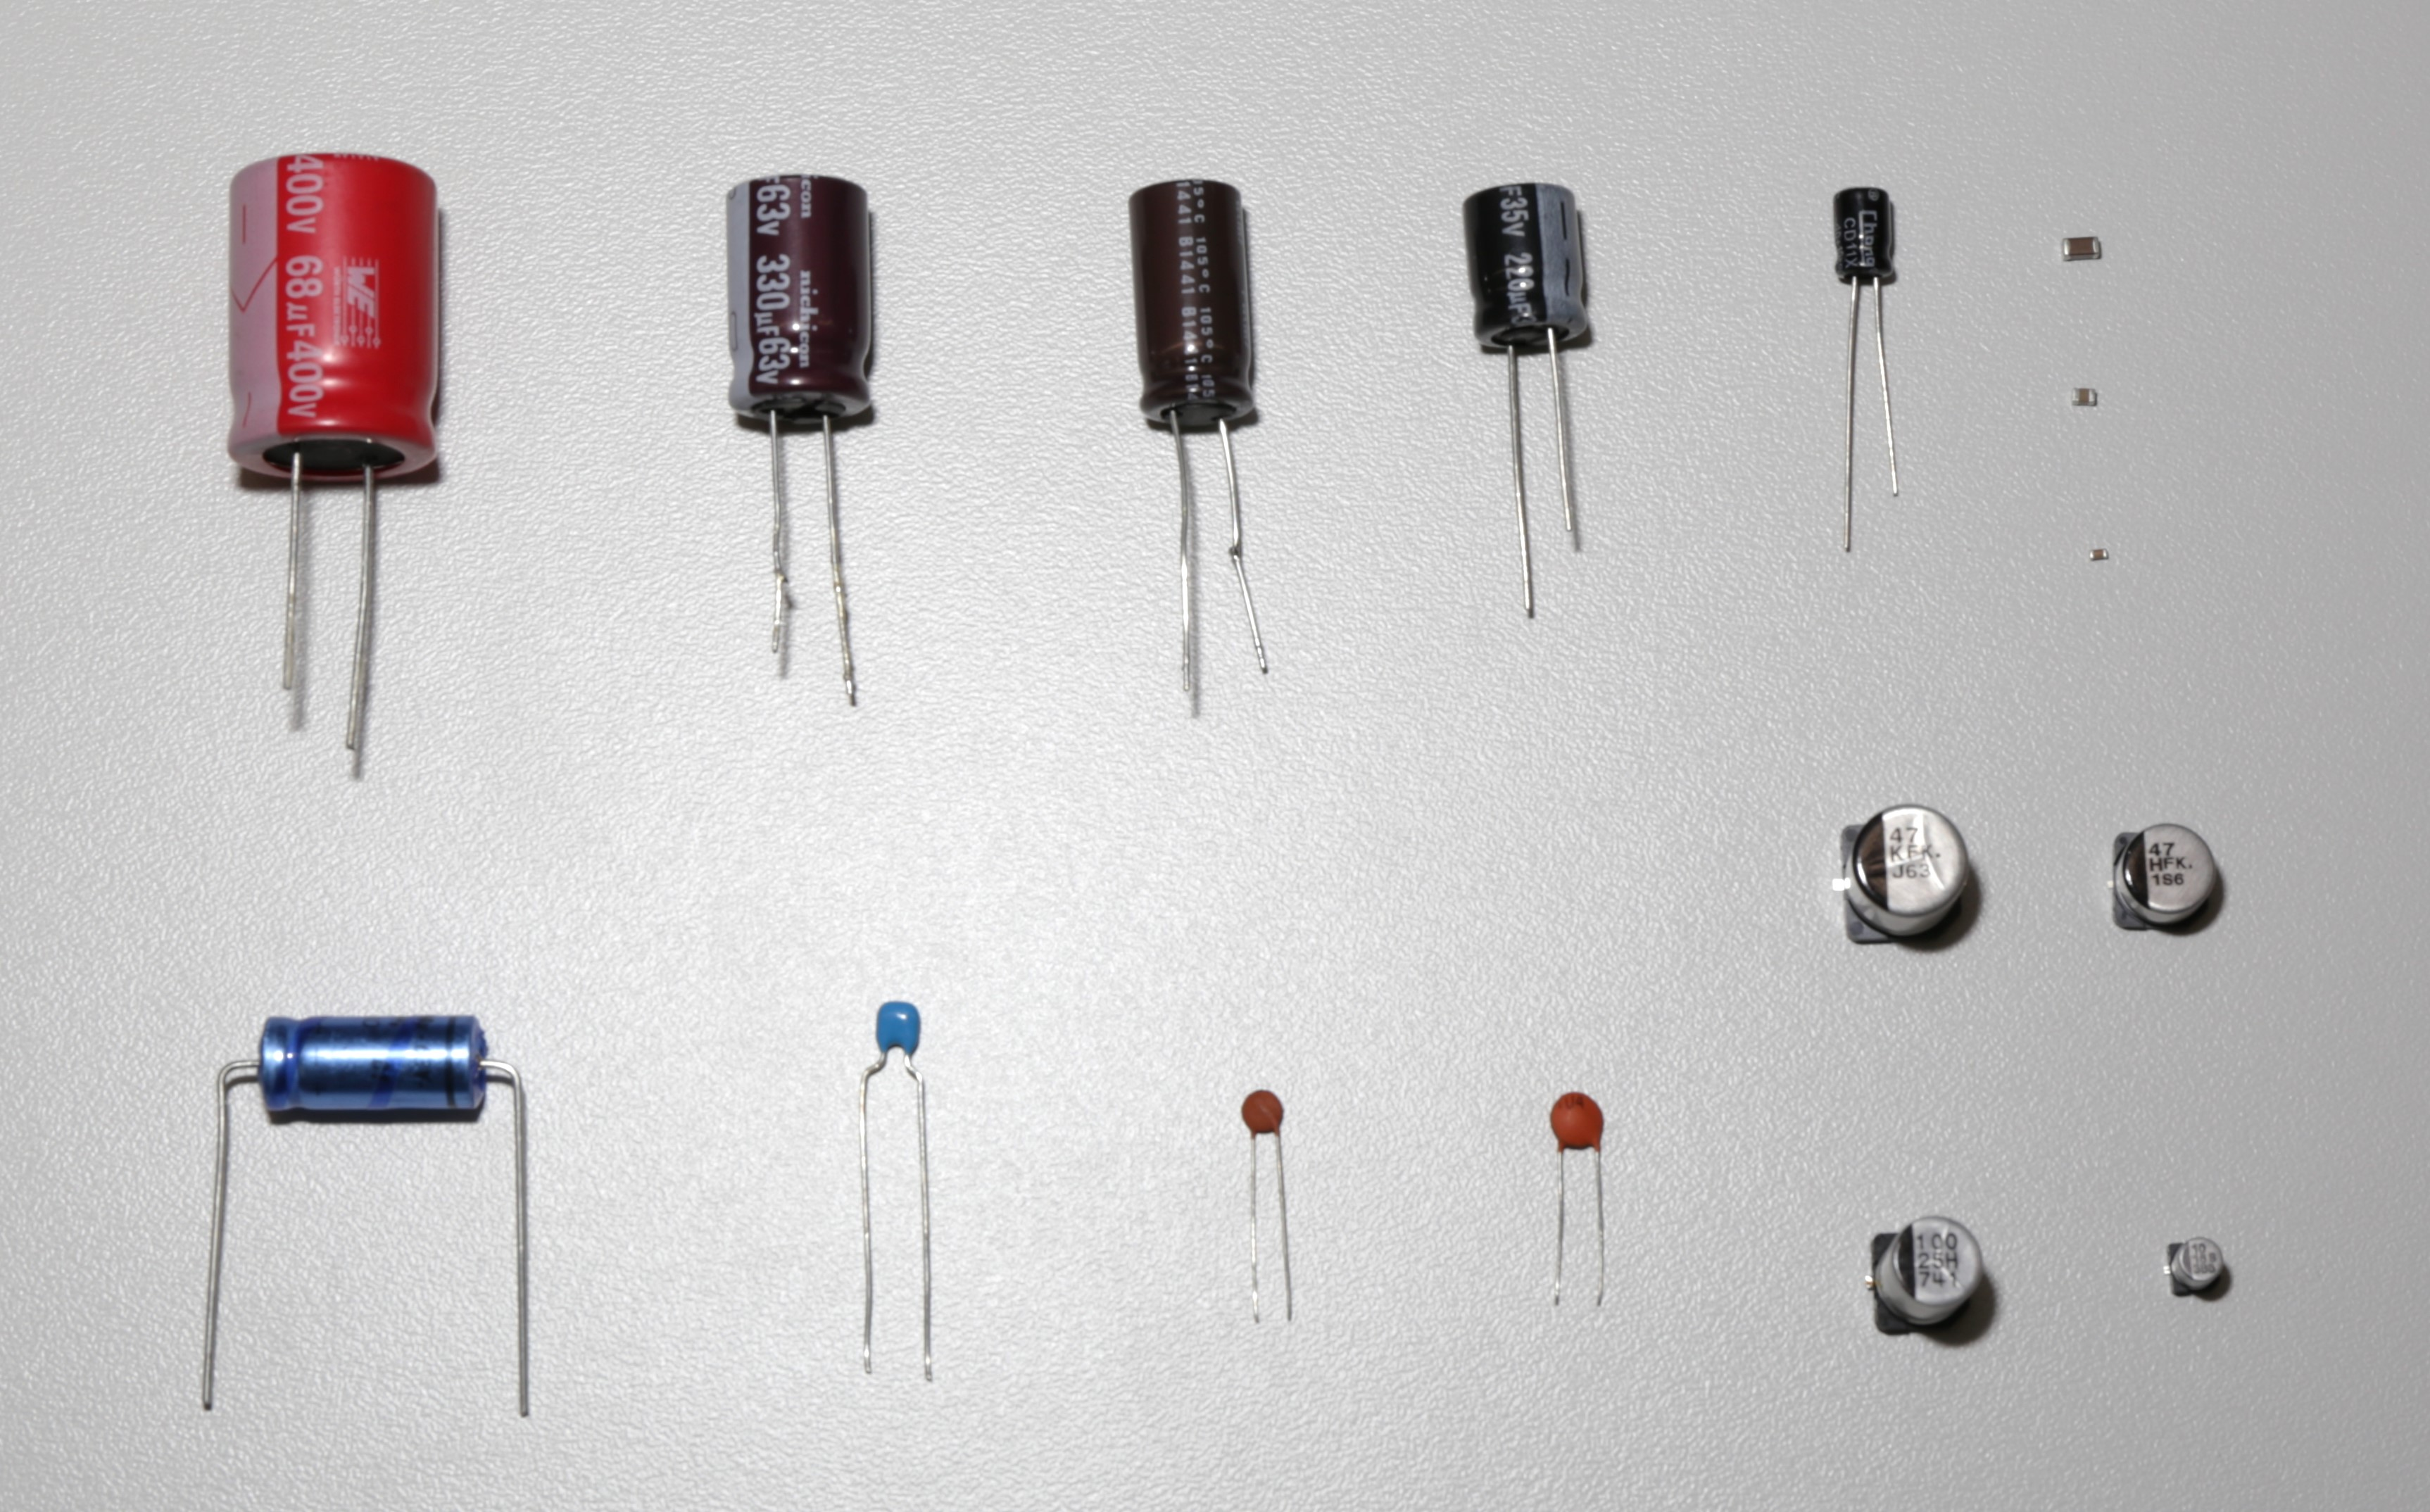
\includegraphics[width=0.7\textwidth]{ko.JPG}
		\s{\caption{\textbf{Verschiedene Arten und Bauformen von Kondensatoren.} Darunter Keramik- und Elektrolytkondensatoren.
		 Diese variieren in Größe, Kapazität und Spannung, um unterschiedlichen Anwendungen gerecht zu werden.}}

		\label{fig:Verschiedene Kondensatoren}
	\end{figure}
	\end{frame}
	%%%%%%%%%%%%%%%%%%%%%%%%%%%%%%%%%%%%%%%%%%%%%%%%% Ende - Bild versch. Kondensatoren	 %%%%%%%%%%%%%%%%%%%%%%%%%%%%%%%%%%%%%%%%%%%%%%
\s{
	Darüber hinaus gibt es sie aber auch in deutlich kleineren bzw. deutlich größeren Dimensionen.
	In der Hochfrequenztechnik werden Kapazitäten beispielsweise lediglich durch das Design der Leiterplatten realisiert,
	während Kondensatoren für industrielle oder enegietechnische Anwendungen mehrere Zentimeter bis Meter groß werden können.

	Was alle Kondensatoren verbindet, ist ihre Fähigkeit, die Eigenschaft der Kapazität nutzbar zu machen,
	wie es im folgenden Schaltbild \ref{fig:idealer Kondensator_ESB} dargestellt ist.
	Dieses Schaltbild repräsentiert jedoch nur die idealisierte, nutzbare Kapazität.
}
%%%%%%%%%%%%%%%%%%%%%%%%%%%%%%%%%%%%%%%%%%%%%%%%% Anfang - Schaltzeichen Kapazität U,I	%%%%%%%%%%%%%%%%%%%%%%%%%%%%%%%%%%%%%%%%%%%%%%
\begin{frame}[t]
	\ftx{Der Kondensator als Bauelement}
	% idealer Kondensator
\b{
	\begin{itemize}
	\item Idealer Kondensator
\end{itemize}
\begin{figure}[h]
	\begin{center}
	\begin{circuitikz}
		\draw (-1,0) to[short,o-] (0,0);
		\draw (0,0)   to [C,i,v, name=C, l={$C$}] (0,-2)
					  to [short,-o] (-1,-2);
		\iarrmore{C}{$i_\mathrm{C}(t)$};
		\varrmore{C}{$u_\mathrm{C}(t)$};

	\end{circuitikz}

	\label{fig:idealer Kondensator_ESB}
	\end{center}
	\end{figure}

	\only<2->{

\begin{itemize}
	\item Ersatzschaltbild eines realen Kondensators
\end{itemize}
\begin{figure}[H]
	\begin{center}
	\begin{circuitikz}[european resistors]
		\draw (0,0)   to [C,i,v, name=C,o-, l={$C$}] (2.4,0)
			  (2,0)   to [R,v, name=R, l={$R_\mathrm{s}$}] (4,0)
			  (4,0)   to [L,v, name=L, l={$L_\mathrm{s}$}] (6,0)
			  (6,0)   to [short,-o] (6.25,0);
	\iarrmore{C}{$i_\mathrm{C}(t)$};
	\varrmore{C}{$u_\mathrm{C}(t)$};
	\varrmore{R}{$u_\mathrm{R}(t)$};
	\varrmore{L}{$u_\mathrm{L}(t)$};

	\end{circuitikz}
	\label{fig:realer Kondensator_ESB}
	\end{center}
	\end{figure}
}
}
\end{frame}
\s{
	\begin{figure}[h]
		\begin{center}
		\begin{circuitikz}
			\draw (-1,0) to[short,o-] (0,0);
			\draw (0,0)   to [C,i,v, name=C, l={$C$}] (0,-2)
						  to [short,-o] (-1,-2);
			\iarrmore{C}{$i_\mathrm{C}(t)$};
			\varrmore{C}{$u_\mathrm{C}(t)$};

		\end{circuitikz}
		\caption{\textbf{Schaltelement eines idealen Kondensators.} Zeigt den Spannungsabfall über dem Kondensator und den Stromfluss durch ihn.}

		\label{fig:idealer Kondensator_ESB}
		\end{center}
		\end{figure}

%%%%%%%%%%%%%%%%%%%%%%%%%%%%%%%%%%%%%%%%%%%%%%%%% Ende - Schaltzeichen Kapazität U,I	 %%%%%%%%%%%%%%%%%%%%%%%%%%%%%%%%%%%%%%%%%%%%%%

	Für eine realitätsgetreue Nachbildung der Schaltung ist es wichtig den Kondensator als Bauteil vollständig zu beschreiben.
	Dies wird mit Hilfe eines Ersatzschaltbildes gemacht, welches auch die ungewollten, also parasitären Eigenschaften
	des Bauteils, nachbildet. Abbildung \ref{fig:realer Kondensator_ESB} zeigt ein solches Ersatzschaltbild.

%%%%%%%%%%%%%%%%%%%%%%%%%%%%%%%%%%%%%%%%%%%%%%%%% Anfang - ESB Kondensator	 %%%%%%%%%%%%%%%%%%%%%%%%%%%%%%%%%%%%%%%%%%%%%%
% realer Kondensator


		\begin{figure}[H]
			\begin{center}
			\begin{circuitikz}[european resistors]
				\draw (0,0)   to [C,i,v, name=C,o-, l={$C$}] (2.4,0)
				      (2,0)   to [R,v, name=R, l={$R_\mathrm{s}$}] (4,0)
				      (4,0)   to [L,v, name=L, l={$L_\mathrm{s}$}] (6,0)
					  (6,0)   to [short,-o] (6.25,0);
			\iarrmore{C}{$i_\mathrm{C}(t)$};
			\varrmore{C}{$u_\mathrm{C}(t)$};
			\varrmore{R}{$u_\mathrm{R}(t)$};
			\varrmore{L}{$u_\mathrm{L}(t)$};

			\end{circuitikz}
			\caption{\textbf{Ersatzschaltbild eines realen Kondensators.} Der ideale Kondensator $C$ wird durch eine Serien-Induktivität
			 $L_\mathrm{s}$ und einen Serien-Widerstand $R_\mathrm{s}$ ergänzt, um parasitäre Effekte zu berücksichtigen.}

			\label{fig:realer Kondensator_ESB}
			\end{center}
			\end{figure}
}

%%%%%%%%%%%%%%%%%%%%%%%%%%%%%%%%%%%%%%%%%%%%%%%%% Ende - ESB Kondensator	 %%%%%%%%%%%%%%%%%%%%%%%%%%%%%%%%%%%%%%%%%%%%%%
\s{
	Im Ersatzschaltbild des Kondensators werden nicht nur die nutzbare Kapazität, sondern auch die parasitären Eigenschaften
	berücksichtigt, die in realen Kondensatoren auftreten. Diese parasitären Eigenschaften entstehen beispielsweise durch die
	Induktivität der Anschlüsse und die ohmschen Verluste im Material.
	Das modellierte Ersatzschaltbild ermöglicht es, diese Effekte im Schaltungsentwurf zu berücksichtigen
	und das Schaltverhalten besser vorherzusagen.
}
%%%%%%%%%%%%%%%%%%%%%%%%%%%%%%%%%%%%%%%%%%%%%%%%%%%% Anfang Merksatz - Kondensator %%%%%%%%%%%%%%%%%%%%%%%%%%%%%%%%%%%%%%%%%
\begin{frame}
	\ftx{Merksatz: Der Kondensator als Bauelement}
	\begin {Merksatz}{}
		 Der Kondensator ist der verzweifelte Versuch eine Kapazität nachzubilden.
	\end {Merksatz}
	\end{frame}
%%%%%%%%%%%%%%%%%%%%%%%%%%%%%%%%%%%%%%%%%%%%%%%%%%%% Ende Merksatz - Kondensator %%%%%%%%%%%%%%%%%%%%%%%%%%%%%%%%%%%%%%%%%
%%%%%%%%%%%%%%%%%%%%%%%%%%%%%%%%%%%%%%%%%%%%%%%%% Anfang - Dielektrikum	 %%%%%%%%%%%%%%%%%%%%%%%%%%%%%%%%%%%%%%%%%%%%%%
\subsection{Das Dielektrikum}
\s{
Das Dielektrium ist, wie der Name bereits impliziert, ein dielektrisches, also elektrisch nicht leitfähiges Material.
Da jedes Material aus Atomen besteht und alle Atomrümpfe mit Elektronen versehen sind (Elektronenhülle),
wirkt sich entsprechend auch ein elektrisch nicht leitfähiges Material auf das Verhalten des elektrischen Feldes aus.
Sobald ein solches Material zwischen die Platten eines Kondensators eingefügt wird, ändern sich demnach auch die Eigenschaften des Kondensators.
In Abbildung \ref{fig:idealer Kondensator mit Dielektrikum} ist anhand der unterbrochenen Pfeilung des elektrischen Feldes
das unterschiedliche Verhalten zu erkennen. Die elektrische Flussdichte D ist eine Hilfsgröße, welche materialunabhängig ist,
auf welche in Abschnitt 1.3.4 noch eingegangen wird.
}
%%%%%%%%%%%%%%%%%%%%%%%%%%%%%%%%%%%%%%%%%%%%%%%%% Anfang - Grafik Dielektrikum	 %%%%%%%%%%%%%%%%%%%%%%%%%%%%%%%%%%%%%%%%%%%%%%
\begin{frame}
	\ftx{Das Dielektrikum}
\begin{figure}[H]
	\centering
		\includesvg[width=0.6\textwidth]{Idealer_Plattenkondensator_Dielektrikum.svg}
		\s{\caption{\textbf{Idealer Kondensator mit Dielektrikum.} Der Kondensator besteht aus zwei Platten, zwischen denen sich ein Dielektrikum befindet. Das Dielektrikum
		 ist ein nicht leitendes Material, das die elektrische Feldstärke reduziert und die Kapazität des Kondensators erhöht, indem es die Relative Dielektrizitätskonstante erhört.}}
		\label{fig:idealer Kondensator mit Dielektrikum}
	\end{figure}
\end{frame}
% Vielleicht an dieser Stelle Einschub zu Dielektrikum,
% Permeativität, was das ist, Zusammenhang zum Wellenwiderstand und zur Lichtgeschwindigkeit.

%%%%%%%%%%%%%%%%%%%%%%%%%%%%%%%%%%%%%%%%%%%%%%%%% Ende - Grafik Dielektrikum	 %%%%%%%%%%%%%%%%%%%%%%%%%%%%%%%%%%%%%%%%%%%%%%
\s{
Die Eigenschaften des Dielektrikums sind materialspezifisch und werden durch die Dielektrizitätszahl $\varepsilon_\mathrm{r}$ quantifiziert.
In Tabelle \ref{tab:dielektrizität} sind Beispiele einiger Dielektrika und deren $\varepsilon_\mathrm{r}$, aufgeführt:
}
%%%%%%%%%%%%%%%%%%%%%%%%%%%%%%%%%%%%%%%%%%%%%%%%% Anfang - Tabelle epsylon	 %%%%%%%%%%%%%%%%%%%%%%%%%%%%%%%%%%%%%%%%%%%%%%
\begin{frame}[t]
	\ftx{Das Dielektrikum}
	\b{
		\begin{itemize}
			\item Relative Dielektrizitätszahl verschiedener Materialien
		\end{itemize}
		\vspace{1cm}
	}
%%%%% Dielektrizitätszahl Einfache Tabelle
\begin{table}[H]
\centering
\resizebox{0.3\textwidth}{!}{%
\begin{tabular}{lc}
\toprule
\textbf{Material} & \textbf{\boldmath$\varepsilon_\mathrm{r}$} \\
\midrule
Vakuum & 1 \\
Luft (bei STP) & 1.0006 \\
Kunststoff (PE) & 2.25-2.3 \\
Glas & 3-10 \\
Keramik & 5-300 \\
Silizium & 11.7 \\
Tantaloxid & 25-30 \\
Wasser & 81 \\
\bottomrule
\end{tabular}%
}
\s{\caption{\textbf{Relative Dielektrizitätszahl verschiedener Materialien.} Diese dimensionslose Zahl gibt an,
wie stark das elektrische Feld in einem Material im Vergleich zum Vakuum beeinflusst wird. Sie ist ein Maß für die Fähigkeit des Materials, elektrische Ladung zu speichern.
Materialien mit einer höheren Dielektrizitätszahl erhöhen die Kapazität eines Kondensators, da sie die elektrische Feldstärke im Inneren verringern.}}
\label{tab:dielektrizität}
\end{table}
\end{frame}

%%%%% Kästchen Tabelle

% \begin{table}[H]
%     \centering
%     \begin{tabular}{|l|c|}
%         \hline
%         \textbf{Material} & \textbf{\boldmath$\varepsilon_\mathrm{r}$} \\
%         \hline
%         Vakuum & 1 \\
%         \hline
%         Luft (bei STP) & 1.0006 \\
%         \hline
%         Kunststoff (PE) & 2.25-2.3 \\
%         \hline
%         Glas & 3-10 \\
%         \hline
%         Keramik & 5-300 \\
%         \hline
%         Silizium & 11.7 \\
%         \hline
%         Tantaloxid & 25-30 \\
%         \hline
%         Wasser & 81 \\
%         \hline
%     \end{tabular}
%     \caption{Dielektrizitätszahl verschiedener Materialien}
%     \label{tab:dielektrizität}
% \end{table}
%%%%%%%%%%%%%%%%%%%%%%%%%%%%%%%%%%%%%%%%%%%%%%%%% Ende - Tabelle epsylon	 %%%%%%%%%%%%%%%%%%%%%%%%%%%%%%%%%%%%%%%%%%%%%%
\s{
	Zur vollständigen Beschreibung der Materialeigenschaften des Dielektrikums wird neben der Dielektrizitätszahl noch die elektrische Feldkonstante $\varepsilon_\mathrm{0}$ benötigt.
	Dabei handelt es sich um das dielektrische Verhalten des elektrischen Feldes im Vakuum. Während die Dielektrizitätszahl $\varepsilon_\mathrm{r}$ einheitslos ist,
	bringt die elektrische Feldkonstante die Einheit $\frac{\text{As}}{\text{Vm}}$ mit. Sie wird mit der relativen Dielektrizitätszahl multipliziert was zusammen
	die Dielektrizitätskonstante $\varepsilon$ ergibt.
}
%%%%%%%%%%%%%%%%%%%%%%%%%%%%%%%%%%%%%%%%%%%%%%%%%%%% Anfang Formel epsylon und Legende %%%%%%%%%%%%%%%%%%%%%%%%%%%%%%%%%
\begin{frame}
	\ftx{Das Dielektrikum}
	\b{
		\begin{equation*}
			[\boldsymbol\varepsilon] = 1\,\frac{\text{Farad}}{\text{m}} = 1\, \frac{\text{F}}{\text{m}} = 1\, \frac{\text{As}}{\text{Vm}}
		\end{equation*}
		\vspace{0.1cm}
		\begin{equation*}
			\boldsymbol\varepsilon = \boldsymbol\varepsilon_\mathrm{0} \cdot \boldsymbol\varepsilon_\mathrm{r}
		\end{equation*}
		\begin{align*}
			\boldsymbol\varepsilon &: 			 \text{Dielektrizitätskonstante}\\
			\boldsymbol\varepsilon_\mathrm{0} &: \text{Elektrische Feldkonstante (8.85421878 $\cdot$ 10}^{-12})\\
			\boldsymbol\varepsilon_\mathrm{r} &: \text{Relative Dielektrizitätszahl}\\
		\end{align*}
	}
\end{frame}
\s{

	\begin{equation*}
		[\boldsymbol\varepsilon] = 1\,\frac{\text{Farad}}{\text{m}} = 1\, \frac{\text{F}}{\text{m}} = 1\, \frac{\text{As}}{\text{Vm}}
	\end{equation*}
	\vspace{0.1cm}
	\begin{equation}
		\boldsymbol\varepsilon = \boldsymbol\varepsilon_\mathrm{0} \cdot \boldsymbol\varepsilon_\mathrm{r}
	\end{equation}
	\begin{align*}
		\boldsymbol\varepsilon &: 			 \text{Dielektrizitätskonstante}\\
		\boldsymbol\varepsilon_\mathrm{0} &: \text{Elektrische Feldkonstante (8.85421878 $\cdot$ 10}^{-12})\\
		\boldsymbol\varepsilon_\mathrm{r} &: \text{Relative Dielektrizitätszahl}\\
	\end{align*}



%%%%%%%%%%%%%%%%%%%%%%%%%%%%%%%%%%%%%%%%%%%%%%%%% Ende Formel epsylon und Legende %%%%%%%%%%%%%%%%%%%%%%%%%%%%%%%%%

% \begin{flushleft} und end{fl..} hilft, falls nicht links zentriert
	Mit Hilfe dieser Materialeigenschaften des Dielektrikums und den Dimensionen sowie der Entfernung der Kondensatorplatten,
	kann die Kapazität des Kondensators wie folgt berechnet werden:
}
\begin{frame}
\ftx{ Der Kondensator als Bauelement}
\b{
	\begin{equation*}
		[C] = 1\,\text{F}
	\end{equation*}
	\vspace{0.1cm}
	\begin{equation*}
		C = \frac{\boldsymbol\varepsilon \cdot A}{d}
	\end{equation*}
	\begin{align*}
		A &: \text{Querschnittsfläche des Materials } (\text{m}{^2}) \\
		d &: \text{Abstand der Elektroden (\text{m})}
	\end{align*}

}
\s{
%%%%%%%%%%%%%%%%%%%%%%%%%%%%%%%%%%%%%%%%%%%%%%%%%%%% Anfang Formel C (epsilon) und Legende %%%%%%%%%%%%%%%%%%%%%%%%%%%%%%%%%
\begin{equation*}
	[C] = 1\,\text{F}
\end{equation*}
\vspace{0.1cm}
\begin{equation}
	C = \frac{\boldsymbol\varepsilon \cdot A}{d}
\end{equation}
\begin{align*}
	A &: \text{Querschnittsfläche des Materials } (\text{m}{^2}) \\
	d &: \text{Abstand der Elektroden (\text{m})}
\end{align*}}
%%%%%%%%%%%%%%%%%%%%%%%%%%%%%%%%%%%%%%%%%%%%%%%%%%%% Ende Formel C (epsilon) und Legende %%%%%%%%%%%%%%%%%%%%%%%%%%%%%%%%%
%%%%%%%%%%%%%%%%%%%%%%%%%%%%%%%%%%%%%%%%%%%%%%%%% Anfang - el. Flussdichte	 %%%%%%%%%%%%%%%%%%%%%%%%%%%%%%%%%%%%%%%%%%%%%%
\end{frame}


\subsection{Die elektrische Flussdichte} %$\vec{D}$}

\begin{frame}[t]
\ftx{Die elektrische Flussdichte $\vec{D}$}
\b{
	\begin{equation*}
		\vec{D} = \boldsymbol\varepsilon \cdot \vec{E} + P
		\end{equation*}

		\only<2->{\begin{itemize}
			\item Im statischen Fall kann die Polarisation $P$ oft vernachlässigt werden
		\end{itemize}
		\vspace{2cm}
		}

		\only<3->{
		\begin{equation*}
			[D] = 1\,\frac{\text{Coulomb}}{\text{m}^2} = 1\,\frac{\text{C}}{\text{m}^2} = 1\,\frac{\text{As}}{\text{m}^2}
		\end{equation*}
		\vspace{0.1cm}
		\begin{equation*}
		\vec{D} = \boldsymbol\varepsilon \cdot \vec{E}
		\end{equation*}}
}
\end{frame}
\s{
Die elektrische Flussdichte $\vec{D}$, auch Verschiebungsdichte genannt, steht proportional zum elektrischen Feld $\vec{E}$.
Ihr Vorteil besteht darin, dass sie materialunabhängig ist, was mathematische Vorteile mit sich bringt.

\begin{equation}
\vec{D} = \boldsymbol\varepsilon \cdot \vec{E} + P
\end{equation}

Zusätzlich zur Dielektrizitätskonstanten $\varepsilon$ wird die Polarisation des Mediums $P$ addiert. Sie beschreibt das Polarisationsverhalten, welches im Einschaltvorgang abläuft.
Im statischen Fall kann die Polarisation $P$ oft vernachlässigt werden, was die Gleichung wie folgt vereinfacht.

\begin{equation*}
	[D] = 1\,\frac{\text{Coulomb}}{\text{m}^2} = 1\,\frac{\text{C}}{\text{m}^2} = 1\,\frac{\text{As}}{\text{m}^2}
\end{equation*}
\vspace{0.1cm}
\begin{equation}
\vec{D} = \boldsymbol\varepsilon \cdot \vec{E}
\end{equation}

}

%%%%%%%%%%%%%%%%%%%%%%%%%%%%%%%%%%%%%%%%%%%%%%%%% Ende - el. Flussdichte	 %%%%%%%%%%%%%%%%%%%%%%%%%%%%%%%%%%%%%%%%%%%%%%
%%%%%%%%%%%%%%%%%%%%%%%%%%%%%%%%%%%%%%%%%%%%%%%%% Anfang - Schaltverhalten Kondensator	 %%%%%%%%%%%%%%%%%%%%%%%%%%%%%%%%%%%%%%%%%%%%%%

%%%%%%%%%%%%%%%%%%%%%%%%%%%%%%%%%%%%%%%%%%%%%%%%% Anfang - Mathematik Kondensator	 %%%%%%%%%%%%%%%%%%%%%%%%%%%%%%%%%%%%%%%%%%%%%%
%%%%%%%%%%%%%%%%%%%%%%%%%%%%%%%%%%%%%%%%%%%%%%%%% Anfang - Übergang zu den zeitabhängigen Vorgängen %%%%%%%%%%%%%%%%%%%%%%%%%
\s{
\textbf{Einführung in die zeitabhängige Vorgänge}


Bisher ist bekannt, dass elektrische Felder in leitfähigen Materialien einen Strom $I$ und eine Spannung $U$ verursachen.
Der Strom $I$ und die Spannung $U$ beschreiben die Felder jedoch nur integral, sie werden also als zeitlich konstant angesehen.
Im Gegensatz zum Widerstand $R$ gibt es jedoch Bauteile (Kondensatoren und Spulen), die ein zeitlich veränderliches Verhalten aufweisen.
Der ohm'sche Widerstand $R$ alleine reicht somit nicht aus, um die Verhältnisse bei Netzwerken mit zeitlich veränderlichen Vorgängen zu beschreiben.
Zur Beschreibung dieser zeitabhängigen Verhalten werden die zeitabhängigen Größen $u(t)$ und $i(t)$ verwendet.

Die Herleitung der Zeitabhängigkeiten kann mathematisch folgendermaßen gezeigt werden.
Aus der Formel \ref{eq:cqu} ist bereits die Grundgleichung des Kondensators bekannt:

\begin{equation}
Q = C \cdot U   \label{eq:qcu}
\end{equation}
%%% NEU DAZU %%%
Zur Beschreibung des zeitlichen Verhaltens des Kondensators, wird die Änderung der Ladung über die Zeit betrachtet

\begin{equation}
	\frac{\mathrm{d}Q}{\mathrm{d}t} = C \cdot \frac{\mathrm{d}U}{\mathrm{d}t}
\end{equation}

$\frac{\mathrm{d}Q}{\mathrm{d}t}$ beschreibt die Änderungsrate der Ladung, welche nach dem Grundgesetz der Elektrotechnik dem Strom $i(t)$ entspricht, der in den Kondensator hinein- oder herausfließt.

%%%%%%%%%%%%%%%%
% In Modul 2 wurde vermittelt, dass der Stromfluss auch als Änderung der Ladung pro Zeit angesehen werden kann:

\begin{equation}
\frac{\mathrm{d}Q}{\mathrm{d}t} = i(t)
\end{equation}

Wird nun in der Formel \ref{eq:qcu} die konstante Ladung Q durch die zeitlich veränderliche Größe $i(t)$ ersetzt,
erhält auch die Spannung eine zeitliche Abhängigkeit.

\begin{equation}
	i_\mathrm{c}(t) = C \cdot \frac{\mathrm{d}u_\mathrm{c}(t)}{\mathrm{d}t} \label{eq:ict}
\end{equation}

Durch mathematische Umstellung nach $u_\mathrm{c}(t)$ kann die Spannung in Abhängigkeit des Stromes und der Kapazität dargestellt werden:

\begin{equation}
	u_\mathrm{c}(t) = \frac{1}{C} \cdot \int i_\mathrm{c}(t) \mathrm{d}t \label{eq:uci}
\end{equation}

Aus der Gleichung \ref{eq:ict} folgt unmittelbar, dass sich die Spannung an einer Kapazität nicht schlagartig ändern kann,
da dafür ein unendlich hoher Strom erforderlich wäre.

}
% Folie Einführung in die zeitabhängige Vorgänge
\begin{frame}[t]
	\ftx{Einführung in die zeitabhängige Vorgänge}

\b{

\begin{itemize}
	\item\begin{equation*} Q = C \cdot U \end{equation*}
		%%% NEU DAZU %%%
	\only<2->{
	\item\begin{equation*}
			\frac{\mathrm{d}Q}{\mathrm{d}t} = C \cdot \frac{\mathrm{d}U}{\mathrm{d}t}
		\end{equation*}
	}
		%%%%%%%%%%%%%%%%
		% In Modul 2 wurde vermittelt, dass der Stromfluss auch als Änderung der Ladung pro Zeit angesehen werden kann:
		\only<3->{
	\item\begin{equation*}
		\frac{\mathrm{d}Q}{\mathrm{d}t} = i(t)
		\end{equation*}
		}
		\only<4->{
	\item\begin{equation*}
			i_\mathrm{c}(t) = C \cdot \frac{\mathrm{d}u_\mathrm{c}(t)}{\mathrm{d}t}
		\end{equation*}
		}
		\only<5->{
	\item\begin{equation*}
			u_\mathrm{c}(t) = \frac{1}{C} \cdot \int i_\mathrm{c}(t) \mathrm{d}t
		\end{equation*}
		}

\end{itemize}
}
\end{frame}

%%%% ggf weg
%Im Abschnitt \ref{sec:Induktivität} wird außerdem eingeführt, dass ein elektrischer Strom ein magnetisches Feld bedingt.
%Im Modul 2 wurde bereits erklärt, dass in beiden Feldern Energie gespeichert und transferiert werden kann.

%%%%%%%%%%%%%%%%%%%%%%%%%%%%%%%%%%%%%%%%%%%%%%%%% Ende - Übergang zu den zeitabhängigen Vorgängen %%%%%%%%%%%%%%%%%%%%%%%%%
\subsection{Schaltverhalten eines Kondensators}
\s{
	Das Schaltverhalten beschreibt das Verhalten eines Bauteils bei Änderung der angelegten Spannung.
	Je nachdem ob eine Spannungsquelle ein- oder ausgeschaltet wird, verhalten sich Strom und Spannung am Bauteil
	entsprechend seiner Charakteristika. Zur Analyse des zeitlichen Verhaltens von Bauteilen ist zuerst ein Schaltbild notwendig,
	welches die zu analysierende Schaltung visualisiert. Abbildung \ref{fig:Schaltbild_CR} zeigt ein Schaltbild einer Reihenschaltung
	einer Kapazität $C$ mit einem Widerstand $R$, welche über einen Schalter mit einer Spannung $U_\mathrm{q}$ versorgt werden können.

}
%%%%%%%%%%%%%%%%%%%%%%%%%%%%%%%%%%%%%%%%%%%%%%%%% Ende - Mathematik Kondensator	 %%%%%%%%%%%%%%%%%%%%%%%%%%%%%%%%%%%%%%%%%%%%%%

%%%%%%%%%%%%%%%%%%%%%%%%%%%%%%%%%%%%%%%%%%%%%%%%% Anfang - Schaltbild mit Schalter	 %%%%%%%%%%%%%%%%%%%%%%%%%%%%%%%%%%%%%%%%%%%%%%
\begin{frame}[t]
\ftx{Schaltverhalten eines Kondensators: Aufladen}
\b{

	\begin{minipage}[t]{0.2\textwidth}
		\begin{equation*}
			\bullet \quad I_\mathrm{max} = \frac{U_\mathrm{q}}{R}
	\end{equation*}
	\end{minipage}
	\vspace{-1.5cm}
% Laden eines Kondensators
	\begin{figure}[H]
		\centering
		\begin{subfigure}[h]{0.5\textwidth}
		\centering
			\begin{circuitikz}[scale=0.8]
            \centering
			\draw (0,-0.3) to[V] (0,4.2)
			 -- (1,4.2) to[normal closed switch, l={Schalter wird bei $t_\mathrm{0} = 5\tau$ geöffnet}] (3,4.2)
			 -- (4,4.2);
			\draw (4,4.2)   to [C,i,v, name=C, l={$C$}] (4,2.2);
			\draw (4,0.2) -- (4,-0.2);
			\draw (4,-0.3) -- (0,-0.3);
			\draw (4,2.2)   to [R,v, name=R, l={$R$}] (4,-0.3);
			\draw[-latex, thick, color=cyan] (-0.7,2.55)  to node[midway,left, color=cyan] {$U_\mathrm{q}$}
			(-0.7,1.35);
			\iarrmore{C}{$i(t)$};
			\varrmore{C}{$u_\mathrm{C}(t)$};
			\varrmore{R}{$u_\mathrm{R}(t)$};

			\end{circuitikz}
		\end{subfigure}

%%%%%%%%%%%%%%%%%%%%%%%%%%%%%%%%%%%%%%%%%%%%%%%%% Ende - Schaltbild mit Schalter	 %%%%%%%%%%%%%%%%%%%%%%%%%%%%%%%%%%%%%%%%%%%%%%
%%%%%%%%%%%%%%%%%%%%%%%%%%%%%%%%%%%%%%%%%%%%%%%%% Anfang - Diagramm mit Schalter	 %%%%%%%%%%%%%%%%%%%%%%%%%%%%%%%%%%%%%%%%%%%%%%
\only<2->{
	\begin{subfigure}[b]{1\textwidth}
			\centering
			\begin{tikzpicture}
			\begin{axis} [
				xlabel={Zeit},
				ylabel={\textcolor{cyan}{$U_\mathrm{q}$}/ \textcolor<3->{voltage}{$u_\mathrm{C}(t)$}/ \textcolor<4->{current}{$i(t)$}},
				% ylabel={
				% 	\textcolor{cyan}{$U_\mathrm{q}$}}
				% 	\only<3->{/ \textcolor{voltage}{$u_\mathrm{C}(t)$}}
				% 	\only<4->{/ \textcolor{current}{$i(t)$}},
				xmin=0, xmax=12.5,
				ymin=-0.2, ymax=1.2,
				ytick={0, 0.37, 0.63, 1},
				yticklabels={%
				0,%
				\only<4->{37\%},%
				\only<3->{63\%},%
				100\%
			},
				%yticklabels={0,37\%, 63\%, 100\%},
				xtick={0, 1, 2, 3, 4, 5, 6, 7, 8, 9, 10, 11, 12},
				xticklabels={0, \(\tau\), \(2\tau\), \(3\tau\), \(4\tau\), \(5\tau\), \(6\tau\), \(7\tau\), \(8\tau\), \(9\tau\), \(10\tau\), \(11\tau\), \(12\tau\)},
				width=10cm,
				height=3.5cm,
				axis lines=middle,
				every axis x label/.style={at={(current axis.right of origin)},anchor=west},
				every axis y label/.style={at={(current axis.above origin)},anchor=south},
				font=\small,
				legend style={font=\scriptsize}
			]

			% Rechtecksignal für die Spannung
			\addplot [cyan, thick] coordinates {(0,1) (5,1) (5,0) (12,0)};

			% Spannungskurve eines Kondensators (Ladekurve)
			\only<3->{\addplot [voltage, domain=0:12, samples=100] {ifthenelse(x<0, 0, 1 - exp(-(x)))};}
			\only<4->{\addplot [current, domain=0:12, samples=100] {ifthenelse(x<0, 0,     exp(-(x)))};}


			% Legenden separat für Spannung und Strom
			\only<2->{\legend{ $U_\mathrm{q}$}}
			\only<3->{\legend{ $U_\mathrm{q}$, $u_\mathrm{C}(t)$}}
			\only<4->{\legend{ $U_\mathrm{q}$, $u_\mathrm{C}(t)$, $i(t)$}}


			% Markierung der Zeitkonstanten
			\only<3->{\draw[dashed] (axis cs:1,0) -- (axis cs:1,0.63) node[right] {};}
			\only<4->{\draw[dashed] (axis cs:1,0) -- (axis cs:1,0.37) node[right] {};}
			\only<4->{\draw[dashed] (axis cs:0,0.37) -- (axis cs:1,0.37) node[right] {};}
			\only<3->{\draw[dashed] (axis cs:0,0.63) -- (axis cs:1,0.63) node[right] {};}
			\node[right] at (5,0.5) {$t_\mathrm{0}$};

			% Punkte zur Hervorhebung
			\only<3->{\addplot[
					only marks,
					mark=*,
					mark options={scale=0.7, fill=black}
				]  coordinates {
					(1, 0.63)

				};}
				\only<4->{\addplot[
					only marks,
					mark=*,
					mark options={scale=0.7, fill=black}
				]  coordinates {
					(1, 0.37)

				};}


			\end{axis}
			\end{tikzpicture}
		\end{subfigure}}
		\end{figure}
}
\end{frame}
%%%%% Laden eines Kondensators
\s{
	\begin{figure}[H]
		\centering
		\begin{subfigure}[h]{0.9\textwidth}
		\centering
			\begin{circuitikz}[scale=0.8]
            \centering
			\draw (0,-0.3) to[V] (0,4.2)
			 -- (1,4.2) to[normal closed switch, l={Schalter wird bei $t_\mathrm{0} = 5\tau$ geöffnet}] (3,4.2)
			 -- (4,4.2);
			\draw (4,4.2)   to [C,i,v, name=C, l={$C$}] (4,2.2);
			\draw (4,0.2) -- (4,-0.2);
			\draw (4,-0.3) -- (0,-0.3);
			\draw (4,2.2)   to [R,v, name=R, l={$R$}] (4,-0.3);
			\draw[-latex, thick, color=cyan] (-0.7,2.55)  to node[midway,left, color=cyan] {$U_\mathrm{q}$}
			(-0.7,1.35);
			\iarrmore{C}{$i(t)$};
			\varrmore{C}{$u_\mathrm{C}(t)$};
			\varrmore{R}{$u_\mathrm{R}(t)$};

			\end{circuitikz}
			\caption{Darstellung der Reihenschaltung bestehend aus einer Kapazität \(C\), einem Widerstand \(R\) und einem Schalter.}
			\label{fig:Schaltbild_CR}
		\end{subfigure}

%%%%%%%%%%%%%%%%%%%%%%%%%%%%%%%%%%%%%%%%%%%%%%%%% Ende - Schaltbild mit Schalter	 %%%%%%%%%%%%%%%%%%%%%%%%%%%%%%%%%%%%%%%%%%%%%%
%%%%%%%%%%%%%%%%%%%%%%%%%%%%%%%%%%%%%%%%%%%%%%%%% Anfang - Diagramm mit Schalter	 %%%%%%%%%%%%%%%%%%%%%%%%%%%%%%%%%%%%%%%%%%%%%%
		\begin{subfigure}[b]{0.9\textwidth}
			\centering
			\begin{tikzpicture}
			\begin{axis} [
				xlabel={Zeit},
				ylabel={\textcolor{cyan}{$U_\mathrm{q}$}/ \textcolor{voltage}{$u_\mathrm{C}(t)$}/ \textcolor{current}{$i(t)$}},
				xmin=0, xmax=12.5,
				ymin=-0.2, ymax=1.2,
				ytick={0, 0.37, 0.63, 1},
				yticklabels={0,37\%, 63\%, 100\%},
				xtick={0, 1, 2, 3, 4, 5, 6, 7, 8, 9, 10, 11, 12},
				xticklabels={0, \(\tau\), \(2\tau\), \(3\tau\), \(4\tau\), \(5\tau\), \(6\tau\), \(7\tau\), \(8\tau\), \(9\tau\), \(10\tau\), \(11\tau\), \(12\tau\)},
				width=10cm,
				height=3.5cm,
				axis lines=middle,
				every axis x label/.style={at={(current axis.right of origin)},anchor=west},
				every axis y label/.style={at={(current axis.above origin)},anchor=south},
				font=\small,
				legend style={font=\scriptsize}
			]

			% Rechtecksignal für die Spannung
			\addplot [cyan, thick] coordinates {(0,1) (5,1) (5,0) (12,0)};

			% Spannungskurve eines Kondensators (Ladekurve)
			\addplot [voltage, domain=0:12, samples=100] {ifthenelse(x<0, 0, 1 - exp(-(x)))};
			\addplot [current, domain=0:12, samples=100] {ifthenelse(x<0, 0,     exp(-(x)))};


			\legend{ $U_\mathrm{q}$ , $u_\mathrm{C}(t)$ , $i(t)$}
			% Markierung der Zeitkonstanten
			\draw[dashed] (axis cs:1,0) -- (axis cs:1,0.63) node[right] {};
			\draw[dashed] (axis cs:1,0) -- (axis cs:1,0.37) node[right] {};
			\draw[dashed] (axis cs:0,0.37) -- (axis cs:1,0.37) node[right] {};
			\draw[dashed] (axis cs:0,0.63) -- (axis cs:1,0.63) node[right] {};
			\node[right] at (5,0.5) {$t_\mathrm{0}$};

			% Punkte zur Hervorhebung
				\addplot[
					only marks,
					mark=*,
					mark options={scale=0.7, fill=black}
				] coordinates {
					(1, 0.63)
					%(6, 0.37)
					(1, 0.37)
					%(6, -0.37)
				};

			\end{axis}
			\end{tikzpicture}
			\caption{Spannungs- und Strom verlauf über der Kapazität bei einer Gleichspannung die zum Zeitpunkt $t = 0$ eingeschaltet wird und zum Zeitpunkt $t_\mathrm{0}$ abgeschaltet wird.}
			\label{fig:Spannungsverlauf_CR}
		\end{subfigure}
		\caption{\textbf{Der Spannungs- und Strom verlauf über der Kapazität.} Das Diagramm zeigt die Reaktion der Kapazität auf die plötzliche Änderung der Spannung und
		veranschaulicht das typische Lade verhalten.}
		\label{fig:Gesamtdarstellung}
		\end{figure}
}

%%%%%%%%%%%%%%%%%%%%%%%%%%%%%%%%%%%%%%%%%%%%%%%%% Ende - Diagramm mit Schalter	 %%%%%%%%%%%%%%%%%%%%%%%%%%%%%%%%%%%%%%%%%%%%%%
\s{
	Im Diagramm \ref{fig:Spannungsverlauf_CR} ist zu sehen, dass sich trotz angelegter Gleichspannung $U_\mathrm{q}$ die Spannung $u_\mathrm{c}(t)$
	zeitgleich nicht mitändert, sondern eine Trägheit aufweisen. Dieses zeitlich veränderliche Verhalten wird im Schaltbild \ref{fig:Schaltbild_CR}
	durch die zeitabhängigen Größen $u(t)$ und $i(t)$ ausgedrückt.

	In diesem Beispiel ist der Schalter zu Beginn geschlossen und wird bei $t_\mathrm{0} = 5\tau$ geöffnet.
	Der Kondensator ist anfangs nicht geladen. Im Diagramm ist zu erkennen, dass sich trotzt angelegter Spannung $U_\mathrm{q}$
	die Spannung über der Kapazität $u_\mathrm{C}(t)$ nicht sprunghaft ändert.

	Dieses Einschaltverhalten resultiert aus der Aufladung der Kapazität. Die Ladungsträger müssen sich dafür auf den Kondensatorplatten
	ansammeln. Dies geschieht so lange, bis die Spannung zwischen den Platten der angelegten Spannung der Spannungsquelle entspricht.
	Da die zur Aufladung benötigten Ladungsträger in die Kondensatorplatten wandern müssen, fließt während dieses Vorgangs ein entsprechender Strom $i_\mathrm{C}(t)$.

	Im Fall einer ideal leitenden Schaltung ohne ohm'schen Widerstand, würden sich die Ladungsträger unendlich schnell auf den Kondensatorplatten ansammeln,
	was einem unendlich hohen Strom entsprechen würde. Im realen Fall hat der Kondensator bzw. die Hinleitung zum Kondensator, einen ohm'schen Widerstand,
	welcher die Ladungsträger auf dem Weg zu den Kondensatorplatten ausbremst, also die elektrische Stromstärke reduziert.
	Daraus folgt der maximal mögliche Strom $I_\mathrm{max}$.

	\begin{equation}
		I_\mathrm{max} = \frac{U_\mathrm{q}}{R}
	\end{equation}

	% Da es dabei dennoch zu relativ hohen Stromstärken kommen kann, werden in Schaltungen mit Kondensatoren mit hohen Kapazitäten sogenannten Vorladewiderstand verbaut.
	% Deren Aufgabe ist es, den maximalen Strom zu begrenzen.

	Sobald der Schalter geöffnet wird, bleibt die Spannung über der Kapazität erhalten.
	Dies bedeutet, dass die zugeführte Energie in der Kapazität verbleibt und sich im stationären Fall nicht mehr ändert.
	Dementsprechend fließt bei einer aufgeladenen Kapazität auch kein Strom mehr, was in einem eingeschwungenen Gleichstromnetzwerk einem Leerlauf gleichzusetzen ist.

	Mit Hilfe der beiden Formeln \ref{eq:ict} und \ref{eq:uci} ist das Verhalten von Strom und Spannung an einer Kapazität vollständig beschrieben,
	was nun diverse Berechnungen ermöglicht. Ein weiteres Beispiel ist das Schaltverhalten einer Kapazität bei anlegen einer Rechteckspannung.
	Der Unterschied besteht darin, dass nicht wie in Beispiel \ref{fig:Schaltbild_CR}, eine konstante Spannungsquelle über einen Schalter geschaltet wird,
	sondern die Spannungsquelle selbst die Eingangsspannung bestimmt.
}
%%%%%%%%%%%%%%%%%%%%%%%%%%%%%%%%%%%%%%%%%%%%%%%%% Anfang - Schaltbild mit Rechteck	 %%%%%%%%%%%%%%%%%%%%%%%%%%%%%%%%%%%%%%%%%%%%%%
\begin{frame}[t]
	\ftx{Schaltverhalten eines Kondensators: Entladen}
	\b{
%%%%% Laden- entladen eines Kondensators
\begin{figure}[H]
	\centering
	\begin{subfigure}[h]{1\textwidth}
	\centering
		\begin{circuitikz}[scale=0.8]
		 \centering
		\draw (0,2.53) -- (0,4.2);
		\draw [thick](0,2) circle (0.54);
		\draw [thick](-0.3,1.8) -- (-0.15,1.8) -- (-0.15,2.2) -- (0.15, 2.2) -- (0.15, 1.8) -- (0.3, 1.8);
		\draw (0,1.45) -- (0,-0.3);
		\draw (4,4.2)   to [C,i,v, name=C, l={$C$}] (4,2.2);
		\draw (0,4.2) -- (4,4.2);
		\draw (4,-0.3) -- (0,-0.3);
		\draw (4,2.2)   to [R,v, name=R, l={$R$}] (4,-0.3);
		\draw[-latex, thick, color=cyan] (-0.7,2.6)  to node[midway,left, color=cyan] {$u(t)$}
		(-0.7,1.4);
		\iarrmore{C}{$i(t)$};
		\varrmore{C}{$u_\mathrm{C}(t)$};
		\varrmore{R}{$u_\mathrm{R}(t)$};

		\end{circuitikz}
	\end{subfigure}
%%%%%%%%%%%%%%%%%%%%%%%%%%%%%%%%%%%%%%%%%%%%%%%%% Ende - Schaltbild mit Rechteck	 %%%%%%%%%%%%%%%%%%%%%%%%%%%%%%%%%%%%%%%%%%%%%%
%%%%%%%%%%%%%%%%%%%%%%%%%%%%%%%%%%%%%%%%%%%%%%%%% Anfang - Diagramm mit Rechteck	 %%%%%%%%%%%%%%%%%%%%%%%%%%%%%%%%%%%%%%%%%%%%%%
	\only<2->{
	\begin{subfigure}[b]{1\textwidth}
		\centering
		\begin{tikzpicture}
		\begin{axis} [
			xlabel={Zeit},
			ylabel={\textcolor{cyan}{$u(t)$}/ \textcolor<3->{voltage}{$u_\mathrm{C}(t)$}/ \textcolor<5->{current}{$i(t)$}},
			xmin=0, xmax=12.5,
			ymin=-1.2, ymax=1.2,
			ytick={-1,-0.63,-0.37,0, 0.37, 0.63, 1},
			yticklabels={
				-100\%, \only<6->{-63\%}, \only<6->{-37\%},
				0, \only<4->{37\%}, \only<3->{63\%}, 100\%
			},
			xtick={0, 1, 2, 3, 4, 5, 6, 7, 8, 9, 10, 11, 12},
			xticklabels={0, \(\tau\), \(2\tau\), \(3\tau\), \(4\tau\), \(5\tau\), \(6\tau\), \(7\tau\), \(8\tau\),
			 \(9\tau\), \(10\tau\), \(11\tau\), \(12\tau\)},
			width=10cm,
			height=5cm,
			axis lines=middle,
			every axis x label/.style={at={(current axis.right of origin)},anchor=west},
			every axis y label/.style={at={(current axis.above origin)},anchor=south},
			font=\small,
			legend style={font=\scriptsize}
			]



		% Rechtecksignal für die Spannung
		\addplot [cyan, thick] coordinates {(0,1) (5,1) (5,0) (12,0)};

		% Spannungskurve eines Kondensators (Ladekurve)
		\only<3->{\addplot [voltage, domain=0:5, samples=100] {ifthenelse(x<0, 0, 1 - exp(-(x)))};}
		\only<5->{\addplot [current, domain=0:5, samples=100] {ifthenelse(x<0, 0,     exp(-(x)))};}

		% Spannungskurve eines Kondensators (Entladekurve)
		\only<4->{\addplot [voltage, domain=5:12, samples=100] {ifthenelse(x<5, 0, exp(-(x-5)))};}
		\only<6->{\addplot [current, domain=5:12, samples=100] {ifthenelse(x<5, 0,-exp(-(x-5)))};}

		 % Legende mit nur selektiv sichtbaren Einträgen
		% Legenden separat für Spannung und Strom
		\only<2->{\legend{ $u(t)$}}
		\only<3->{\legend{ $u(t)$, $u_\mathrm{C}(t)$}}
		\only<4->{\legend{ $u(t)$, $u_\mathrm{C}(t)$}}
		\only<5->{\legend{ $u(t)$, $u_\mathrm{C}(t)$, $i(t)$}}
		\only<6->{\legend{ $u(t)$, $u_\mathrm{C}(t)$, $i(t)$}}

		 % Markierungen der Zeitkonstanten
		 \only<3->{\draw[dashed] (axis cs:1,0) -- (axis cs:1,0.63) node[right] {};}
		 \only<4->{\draw[dashed] (axis cs:6,0) -- (axis cs:6,0.37) node[right] {};}
		 \only<3->{\draw[dashed] (axis cs:1,0) -- (axis cs:1,0.37) node[right] {};}
		 \only<6->{\draw[dashed] (axis cs:6,-1) -- (axis cs:6,-0.37) node[right] {};}
		 \only<5->{\draw[dashed] (axis cs:0,0.37) -- (axis cs:1,0.37) node[right] {};}
		 \only<3->{\draw[dashed] (axis cs:0,0.63) -- (axis cs:1,0.63) node[right] {};}
		 \only<6->{\draw[dashed] (axis cs:0,-0.37) -- (axis cs:6,-0.37) node[right] {};}
		 \only<4->{\draw[dashed] (axis cs:0,0.37) -- (axis cs:6,0.37) node[right] {};}
		 \only<6->{\draw [dashed] (axis cs:0,-1) -- (axis cs:12,-1);}
		 \only<3->{\draw [dashed] (axis cs:5,1) -- (axis cs:12,1);}

		% Punkte zur Hervorhebung
		\only<3->{\addplot[
			only marks,
			mark=*,
			mark options={scale=0.7, fill=black}
		] coordinates {
			(1, 0.63)
		};}
		\only<5->{\addplot[
			only marks,
			mark=*,
			mark options={scale=0.7, fill=black}
		] coordinates {
			(1, 0.37)
		};}
		\only<4->{\addplot[
			only marks,
			mark=*,
			mark options={scale=0.7, fill=black}
		] coordinates {
			(6, 0.37)
		};}
		\only<6->{\addplot[
			only marks,
			mark=*,
			mark options={scale=0.7, fill=black}
		] coordinates {
			(6, -0.37)
		};}

		\end{axis}
		\end{tikzpicture}
	\end{subfigure}}
	\end{figure}

}
\end{frame}
\s{
%%%%% Laden- entladen eines Kondensators
	\begin{figure}[H]
		\centering
		\begin{subfigure}[h]{0.85\textwidth}
		\centering
			\begin{circuitikz}[scale=0.8]
             \centering
			\draw (0,2.53) -- (0,4.2);
			\draw [thick](0,2) circle (0.54);
			\draw [thick](-0.3,1.8) -- (-0.15,1.8) -- (-0.15,2.2) -- (0.15, 2.2) -- (0.15, 1.8) -- (0.3, 1.8);
			\draw (0,1.45) -- (0,-0.3);
			\draw (4,4.2)   to [C,i,v, name=C, l={$C$}] (4,2.2);
			\draw (0,4.2) -- (4,4.2);
			\draw (4,-0.3) -- (0,-0.3);
			\draw (4,2.2)   to [R,v, name=R, l={$R$}] (4,-0.3);
			\draw[-latex, thick, color=cyan] (-0.7,2.6)  to node[midway,left, color=cyan] {$u(t)$}
			(-0.7,1.4);
			\iarrmore{C}{$i(t)$};
			\varrmore{C}{$u_\mathrm{C}(t)$};
			\varrmore{R}{$u_\mathrm{R}(t)$};

			\end{circuitikz}
			\caption{Darstellung der Reihenschaltung bestehend aus einer Kapazität \(C\) und einem Widerstand \(R\) an einer rechteckförmigen Spannungsquelle.}
			\label{fig:Schaltbild_CRR}
		\end{subfigure}
%%%%%%%%%%%%%%%%%%%%%%%%%%%%%%%%%%%%%%%%%%%%%%%%% Ende - Schaltbild mit Rechteck	 %%%%%%%%%%%%%%%%%%%%%%%%%%%%%%%%%%%%%%%%%%%%%%
%%%%%%%%%%%%%%%%%%%%%%%%%%%%%%%%%%%%%%%%%%%%%%%%% Anfang - Diagramm mit Rechteck	 %%%%%%%%%%%%%%%%%%%%%%%%%%%%%%%%%%%%%%%%%%%%%%
		\begin{subfigure}[b]{0.9\textwidth}
			\centering
			\begin{tikzpicture}
			\begin{axis} [
				xlabel={Zeit},
				ylabel={\textcolor{cyan}{$u(t)$}/ \textcolor{voltage}{$u_\mathrm{C}(t)$}/ \textcolor{current}{$i(t)$}},
				xmin=0, xmax=12.5,
				ymin=-1.2, ymax=1.2,
				ytick={-1,-0.63,-0.37,0, 0.37, 0.63, 1},
				yticklabels={-100\%,-63\%,-37\%,0,37\%, 63\%, 100\%},
				xtick={0, 1, 2, 3, 4, 5, 6, 7, 8, 9, 10, 11, 12},
				xticklabels={0, \(\tau\), \(2\tau\), \(3\tau\), \(4\tau\), \(5\tau\), \(6\tau\), \(7\tau\), \(8\tau\), \(9\tau\), \(10\tau\), \(11\tau\), \(12\tau\)},
				width=10cm,
				height=5cm,
				axis lines=middle,
				every axis x label/.style={at={(current axis.right of origin)},anchor=west},
				every axis y label/.style={at={(current axis.above origin)},anchor=south},
				font=\small,
				legend style={font=\scriptsize}
				]



			% Rechtecksignal für die Spannung
			\addplot [cyan, thick] coordinates {(0,1) (5,1) (5,0) (12,0)};

			% Spannungskurve eines Kondensators (Ladekurve)
			\addplot [voltage, domain=0:5, samples=100] {ifthenelse(x<0, 0, 1 - exp(-(x)))};
			\addplot [current, domain=0:5, samples=100] {ifthenelse(x<0, 0,     exp(-(x)))};

			% Spannungskurve eines Kondensators (Entladekurve)
			\addplot [voltage, domain=5:12, samples=100] {ifthenelse(x<5, 0, exp(-(x-5)))};
			\addplot [current, domain=5:12, samples=100] {ifthenelse(x<5, 0,-exp(-(x-5)))};

			\legend{ $u(t)$ , $u_\mathrm{C}(t)$ , $i(t)$}
			% Markierung der Zeitkonstanten
			\draw[dashed] (axis cs:1,0) -- (axis cs:1,0.63) node[right] {};
			\draw[dashed] (axis cs:6,0) -- (axis cs:6,0.37) node[right] {};
			\draw[dashed] (axis cs:1,0) -- (axis cs:1,0.37) node[right] {};
			\draw[dashed] (axis cs:6,-1) -- (axis cs:6,-0.37) node[right] {};
			\draw[dashed] (axis cs:0,0.37) -- (axis cs:1,0.37) node[right] {};
			\draw[dashed] (axis cs:0,0.63) -- (axis cs:1,0.63) node[right] {};
			\draw[dashed] (axis cs:0,-0.37) -- (axis cs:6,-0.37) node[right] {};
			\draw[dashed] (axis cs:0,0.37) -- (axis cs:6,0.37) node[right] {};
			\draw [dashed] (axis cs:0,-1) -- (axis cs:12,-1);
            \draw [dashed] (axis cs:5,1) -- (axis cs:12,1);

			% Punkte zur Hervorhebung
				\addplot[
					only marks,
					mark=*,
					mark options={scale=0.7, fill=black}
				] coordinates {
					(1, 0.63)
					(6, 0.37)
					(1, 0.37)
					(6, -0.37)
				};

			\end{axis}
			\end{tikzpicture}
			\caption{Spannungs- und Strom verlauf über der Kapazität bei einer rechteckförmigen Spannung.}
			\label{fig:Spannungsverlauf}
		\end{subfigure}
		\caption{\textbf{Spannungs- und Stromverlauf über der Kapazität.} Das Diagramm zeigt die Reaktion der Kapazität auf eine plötzliche Änderung
		 der Spannung und veranschaulicht das typische Lade- und Entladeverhalten des Kondensators.}
		\label{fig:Gesamtdarstellung}
		\end{figure}
}% Nur Skript

%%%%%%%%%%%%%%%%%%%%%%%%%%%%%%%%%%%%%%%%%%%%%%%%% Ende - Diagramm mit Rechteck	 %%%%%%%%%%%%%%%%%%%%%%%%%%%%%%%%%%%%%%%%%%%%%%
\s{
	Im Gegensatz zum Schalter, versucht die Spannungsquelle im Beispiel \ref{fig:Schaltbild_CRR}
	ab dem Zeitpunkt $t_\mathrm{0} = 5\tau$ die Systemspannung auf $0$ zu ziehen. Dies führt dazu,
	dass die Kapazität entladen wird. Dies führt entsprechend zu einem entgegengesetzten Stromfluss $i_\mathrm{C}(t)$,
	da sich die Ladungsträger von den Kondensatorplatten wegbewegen, um wieder einen neutralen Zustand zu erreichen.
	%Neben der Verwendung zur Energiespeicherung, werden Kondensatoren auch für die Filterung von Frequenzen, zur Zeitmessung oder für die Signalverarbeitung genutzt.
}
%%%%%%%%%%%%%%%%%%%%%%%%%%%%%%%%%%%%%%%%%%%%%%%%% Ende - Schaltverhalten Kondensator	 %%%%%%%%%%%%%%%%%%%%%%%%%%%%%%%%%%%%%%%%%%%%%%
%%%%%%%%%%%%%%%%%%%%%%%%%%%%%%%% Anfang - Beispiel Rechnung Kondensator %%%%%%%%%%%%%%%%%%%%%%%%%%%%%%%
\begin{frame}
	\ftx{Beispielrechnung Kapazität}
\begin{bsp}{Berechnungs der Kapazität}{}
\begin{itemize}

	\item Ladung auf Platten $Q = \sigma \cdot A = \varepsilon \cdot E \cdot A$
	\item Kapazität mit $C = \frac{\varepsilon \cdot A}{d}$ berechnen
	\item Gespeicherte Energie $W = \frac{1}{2} \cdot C \cdot V^2 $
	\item Kapazität zweier Kondensatoren mit verschiedenen $\varepsilon_{\mathrm{r}}$ über $\vec{D}$ berechnen

\end{itemize}
\end{bsp}

\end{frame}
%%%%%%%%%%%%%%%%%%%%%%%%%%%%%%%% Ende - Beispiel Rechnung Kondensator %%%%%%%%%%%%%%%%%%%%%%%%%%%%%%%
